% Shared standalone design for the editable figure reconstructions.
\documentclass[tikz,border=5pt,10pt]{standalone}
\usepackage[T1]{fontenc}
\usepackage[utf8]{inputenc}
\usepackage{newpxtext,newpxmath}
\usepackage[scaled=.94]{sourcesanspro}
\usepackage{pgfplots}
\pgfplotsset{compat=1.18}
\usetikzlibrary{arrows.meta,calc,positioning,decorations.pathreplacing,
  decorations.markings,patterns,matrix,shapes.geometric,fit,backgrounds,
  intersections,angles,quotes}
\definecolor{ink}{HTML}{203746}
\definecolor{accent}{HTML}{146C78}
\definecolor{muted}{HTML}{667780}
\definecolor{signalred}{HTML}{B94B44}
\color{ink}
\tikzset{>=Latex,line width=.8pt,
  every node/.style={font=\small},
  axis/.style={->,draw=muted,line width=.5pt},
  guide/.style={draw=muted,dashed,line width=.45pt},
  curve/.style={draw=accent,line width=1pt},
  marker/.style={circle,fill=accent,inner sep=1.5pt},
  labelbox/.style={fill=white,inner sep=2pt}}

\begin{document}
\begin{tikzpicture}[x=1.2cm,y=1cm]
\pgfmathdeclarefunction{signal}{1}{\pgfmathparse{1.5+.5*sin(55*#1)+.25*cos(170*#1)+.15*sin(690*#1)+.07*cos(1410*#1)}}
\pgfmathdeclarefunction{average}{1}{\pgfmathparse{1.5+.5*sin(27.5)/(55*pi/360)*sin(55*#1)+.25*sin(85)/(170*pi/360)*cos(170*#1)+.15*sin(345)/(690*pi/360)*sin(690*#1)+.07*sin(705)/(1410*pi/360)*cos(1410*#1)}}
\draw[axis] (0,0)--(9.7,0) node[right] {$t$};
\draw[axis] (0,-.08)--(0,2.65);
\fill[accent!9] (4,0) rectangle (5,2.55);
\draw[ink,line width=.65pt,domain=0:9.2,samples=1100] plot (\x,{signal(\x)});
\draw[signalred,dashed,line width=1.1pt,domain=0:9.2,samples=320] plot (\x,{average(\x)});
\foreach \x in {4,4.5,5}{\draw[guide] (\x,0)--(\x,2.55);}
\node[below left] at (4,-.12) {$x-\tfrac12$};\node[below right] at (5,-.12) {$x+\tfrac12$};
\node[above] at (4.5,2.55) {$x$};
\fill[signalred] (4.5,{average(4.5)}) circle(1.8pt);
\node[anchor=west,ink] at (6.1,3.15) {$f$};\draw[ink] (5.35,3.15)--(5.95,3.15);
\node[anchor=west,signalred] at (7.8,3.15) {$f\star\mathbf1_{[-1/2,1/2]}$};\draw[signalred,dashed,thick] (7.05,3.15)--(7.65,3.15);
\node at (4.7,-1.15) {$\displaystyle(f\star\mathbf1_{[-1/2,1/2]})(x)=\int_{x-1/2}^{x+1/2}f(t)\,\mathrm dt$};
\end{tikzpicture}
\end{document}
